\documentclass[aspectratio=169,10pt]{beamer}

\usepackage[utf8]{inputenc}
\usepackage[T1]{fontenc}
\usepackage[spanish]{babel}
\usepackage{lmodern}
\usepackage{graphicx}
\usepackage{booktabs}
\usepackage{tikz}
\usepackage{amsmath}
\usepackage{microtype}
\usetikzlibrary{arrows.meta, positioning, fit}

\graphicspath{{../article/}{./}}

\definecolor{ULLNavy}{HTML}{3C045B}
\definecolor{ULLBlue}{HTML}{718B82}
\definecolor{ULLGold}{HTML}{BDA873}
\definecolor{Ink}{HTML}{302838}
\definecolor{Mist}{HTML}{F5F3F6}
\definecolor{Muted}{HTML}{71677B}
\definecolor{Positive}{HTML}{16836B}
\definecolor{Alert}{HTML}{B86646}

\usetheme{default}
\usecolortheme{default}
\setbeamercolor{normal text}{fg=Ink,bg=white}
\setbeamercolor{structure}{fg=ULLNavy}
\setbeamercolor{frametitle}{fg=ULLNavy,bg=white}
\setbeamercolor{title}{fg=white}
\setbeamercolor{subtitle}{fg=white!82}
\setbeamercolor{block title}{fg=white,bg=ULLNavy}
\setbeamercolor{block body}{fg=Ink,bg=Mist}
\setbeamercolor{alerted text}{fg=ULLBlue}
\setbeamerfont{title}{size=\LARGE,series=\bfseries}
\setbeamerfont{frametitle}{size=\large,series=\bfseries}
\setbeamertemplate{navigation symbols}{}
\setbeamertemplate{itemize item}{\color{ULLBlue}\raisebox{0.2ex}{\scriptsize$\blacktriangleright$}}
\setbeamertemplate{itemize subitem}{\color{ULLGold}\raisebox{0.2ex}{\tiny$\blacktriangleright$}}
\setbeamertemplate{caption}{\raggedright\insertcaption\par}
\setbeamersize{text margin left=1.05cm,text margin right=1.05cm}
\newcommand{\contentframetotal}{9}
\setbeamertemplate{footline}{%
  \begin{beamercolorbox}[wd=\paperwidth,ht=.76cm,dp=0cm]{normal text}
    \begin{tikzpicture}[remember picture,overlay]
      \fill[ULLNavy,rounded corners=2pt]
        ([xshift=1.05cm,yshift=.12cm]current page.south west)
        rectangle
        ([xshift=3.65cm,yshift=.64cm]current page.south west);
      \node at ([xshift=2.35cm,yshift=.38cm]current page.south west)
        {
\includegraphics[width=1.9cm]{ull-logo-white.png}};
      \pgfmathsetmacro{\progressratio}{min(1,\insertframenumber/\contentframetotal)}
      \draw[Muted!20,line width=3pt,line cap=round]
        ([xshift=4.15cm,yshift=.38cm]current page.south west) --
        ([xshift=13.75cm,yshift=.38cm]current page.south west);
      \draw[ULLBlue,line width=3pt,line cap=round]
        ([xshift=4.15cm,yshift=.38cm]current page.south west) --
        ([xshift={4.15cm+9.6cm*\progressratio},yshift=.38cm]current page.south west);
      \node[anchor=east,text=ULLNavy,font=\scriptsize\bfseries]
        at ([xshift=-1.05cm,yshift=.38cm]current page.south east)
        {\insertframenumber/\contentframetotal};
    \end{tikzpicture}
  \end{beamercolorbox}%
}
\setbeamertemplate{frametitle}{%
  \vspace{0.45em}%
  \insertframetitle\par
  \vspace{0.15em}%
  {\color{ULLBlue}\rule{0.12\paperwidth}{1.4pt}}%
  \vspace{0.3em}%
}
\setlength{\leftmargini}{1.25em}
\setlength{\parskip}{0.25em}

\newcommand{\metric}[2]{%
  \begin{beamercolorbox}[wd=\linewidth,sep=0.32em,rounded=true]{block body}
    {\color{ULLBlue}\large\bfseries #1}\par
    {\scriptsize\color{Muted}#2}
  \end{beamercolorbox}
}
\newcommand{\tagline}[1]{{\color{ULLBlue}\bfseries #1}}

\title{Recalibración espectrofotométrica de Gaia DR3}
\subtitle{Una red neuronal informada por la física y referencias CALSPEC}
\author{Yaiza María Martín Mesones}
\institute{Prácticas externas \textbar\ Instituto de Astrofísica de Canarias\\Universidad de La Laguna}
\date{Curso 2026/2027}

\begin{document}

\begin{frame}[plain]
  \begin{tikzpicture}[remember picture,overlay]
    \fill[ULLNavy] (current page.south west) rectangle (current page.north east);
    \fill[ULLNavy!88!ULLBlue] (current page.south east) -- ++(-5.7,0) -- ++(5.7,3.5) -- cycle;
    \fill[ULLGold] (current page.north west) rectangle ([xshift=.11cm]current page.south west);
    \node[anchor=north east,align=right,text=ULLGold,font=\small\bfseries]
      at ([xshift=-.95cm,yshift=-.65cm]current page.north east)
      {PRÁCTICAS EXTERNAS\\[-.05cm]
       {\color{white!75}\scriptsize CURSO 2026/2027}};
    \begin{scope}[shift={([xshift=9.45cm,yshift=3.0cm]current page.south west)}]
      \draw[white!25,line width=.5pt] (0,0) -- (5,0);
      \draw[white!25,line width=.5pt] (0,0) -- (0,2.7);
      \draw[white!60,line width=1.25pt]
        plot[smooth,tension=.75] coordinates {
          (0.15,.65) (.65,1.15) (1.05,.9) (1.45,1.55)
          (1.9,1.18) (2.35,2.15) (2.75,1.42) (3.2,1.7)
          (3.6,1.22) (4.15,1.35) (4.85,.72)
        };
      \draw[ULLGold,line width=1pt] (0,0) -- (.5,0);
    \end{scope}
    \node[anchor=north west,inner sep=0pt] at
      ([xshift=1cm,yshift=-1.8cm]current page.north west) {%
        \begin{minipage}[t]{.50\textwidth}
          {\color{ULLGold}\small PRÁCTICAS EXTERNAS EN ASTROFÍSICA\par}
          \vspace{0.2cm}
          {\color{white}\Huge\bfseries GaiaCalibNet\par}
          \vspace{0.12cm}
          {\color{white!86}\large Recalibración de Gaia DR3\\con referencias CALSPEC\par}
          \vspace{0.42cm}
          {\color{white}\normalsize Yaiza María Martín Mesones\par}
          \vspace{0.12cm}
          {\color{white!76}\footnotesize
            Instituto de Astrofísica de Canarias (IAC)\\
            Tutor académico: Teresa de Jesús Bermúdez de León\\
            Tutor en la entidad: Carlos Allende Prieto\par}
        \end{minipage}%
      };
    \node[anchor=south east,text=white!74,font=\small]
      at ([xshift=-1.05cm,yshift=.38cm]current page.south east)
      {
\includegraphics[width=2.85cm]{ull-logo-white.png}};
  \end{tikzpicture}
\end{frame}
\setcounter{framenumber}{0}

\begin{frame}{El reto: pasar de espectros a un flujo fiable}
  \begin{columns}[T,onlytextwidth]
    \column{.57\textwidth}
      \begin{block}{Punto de partida}
        Gaia DR3 ofrece espectros BP/RP para una muestra enorme, pero su
        respuesta instrumental introduce sesgos y oscilaciones.
      \end{block}
      \vspace{0.1em}
      \begin{itemize}
        \setlength{\itemsep}{0.25em}
        \item \textbf{CALSPEC}: espectros observados de referencia.
        \item Corregir Gaia preservando la forma física del espectro.
        \item Equilibrar datos, ruido y restricciones físicas con pocas referencias.
      \end{itemize}
    \column{.38\textwidth}
      \begin{beamercolorbox}[wd=\linewidth,sep=1em,rounded=true]{block body}
        {\color{ULLNavy}\bfseries Relación objetivo}\par\vspace{0.5em}
        \[
          Y_{\mathrm{ref}}(\lambda)
          = X_{\mathrm{Gaia}}(\lambda)\,R(\lambda)
        \]
        {\scriptsize\color{Muted}Estimar una respuesta multiplicativa
        $R(\lambda)>0$ para recuperar el flujo de referencia.}
      \end{beamercolorbox}
      \vspace{0.5em}
      {\scriptsize\color{Muted}La recalibración es relativa a las referencias
      disponibles; no sustituye la calibración oficial de Gaia.}
  \end{columns}
\end{frame}

\begin{frame}{La estancia: investigación aplicada en el IAC}
  \begin{columns}[T,onlytextwidth]
    \column{.59\textwidth}
      \begin{itemize}
        \item \textbf{Periodo:} 10 de julio--7 de septiembre; \textbf{250 horas}
              presenciales en el área de investigación y espectrografía.
        \item Revisión bibliográfica sobre CALSPEC y los espectros BP/RP de Gaia.
        \item Automatización de ingesta, descarga y cruce de catálogos.
        \item Preparación de espectros comparables y experimentación con
              arquitecturas y funciones de pérdida.
        \item Evaluación, visualización de resultados y exploración de
              generalización con bibliotecas complementarias.
      \end{itemize}
    \column{.36\textwidth}
      \begin{beamercolorbox}[wd=\linewidth,sep=0.85em,rounded=true]{block body}
        {\color{ULLNavy}\bfseries Herramientas}\par\vspace{0.35em}
        Python \textbullet\ PyTorch \textbullet\ NumPy\\
        SciPy \textbullet\ Astropy \textbullet\ GaiaXPy\\
        Git/GitHub \textbullet\ LaTeX
      \end{beamercolorbox}
      \vspace{0.65em}
      \begin{beamercolorbox}[wd=\linewidth,sep=0.85em,rounded=true]{block body}
        {\color{ULLNavy}\bfseries Competencias en práctica}\par\vspace{0.35em}
        Modelización matemática, análisis de datos reales, validación
        experimental y comunicación científica.
      \end{beamercolorbox}
  \end{columns}
\end{frame}

\begin{frame}{Del catálogo al conjunto de evaluación}
  \centering
  \begin{tikzpicture}[
    node distance=0.48cm and 0.45cm,
    stage/.style={draw=ULLBlue,fill=Mist,rounded corners=2pt,minimum height=1.05cm,
      text width=2.25cm,align=center,font=\footnotesize\bfseries,text=Ink},
    arrow/.style={-{Stealth[length=2mm]},draw=ULLGold,line width=1.1pt}
  ]
    \node[stage] (calspec) {CALSPEC\\referencias};
    \node[stage,right=of calspec] (match) {Cruce con\\Gaia DR3};
    \node[stage,right=of match] (prep) {Homogeneización\\espectral};
    \node[stage,right=of prep] (eval) {76 estrellas\\evaluación};
    \draw[arrow] (calspec) -- (match);
    \draw[arrow] (match) -- (prep);
    \draw[arrow] (prep) -- (eval);
  \end{tikzpicture}
  \vspace{1.1em}
  \begin{columns}[T,onlytextwidth]
    \column{.53\textwidth}
      \begin{itemize}
        \item Cruce astrométrico con corrección de época y filtro fotométrico.
        \item Los espectros CALSPEC se degradan para compararlos con la
              resolución de Gaia XP.
        \item Se preparan flujos, incertidumbres y parámetros estelares.
      \end{itemize}
    \column{.42\textwidth}
      \begin{beamercolorbox}[wd=\linewidth,sep=0.8em,rounded=true]{block body}
        {\color{ULLNavy}\bfseries Validación sin reutilizar la estrella evaluada}\par
        \small Leave-One-Out Cross-Validation: en cada partición se reserva
        una estrella y se entrena con las restantes.
      \end{beamercolorbox}
  \end{columns}
\end{frame}

\begin{frame}{Modelo híbrido: estructura global y corrección local}
  \begin{columns}[T,onlytextwidth]
    \column{.64\textwidth}
      \centering
      \begin{tikzpicture}[
        node distance=0.25cm,
        box/.style={draw=ULLBlue,fill=Mist,rounded corners=2pt,text width=1.65cm,
          minimum height=0.78cm,align=center,font=\scriptsize,text=Ink},
        narrow/.style={draw=ULLGold,fill=white,rounded corners=2pt,text width=1.65cm,
          minimum height=0.68cm,align=center,font=\scriptsize,text=Ink},
        arrow/.style={-{Stealth[length=2mm]},draw=ULLNavy,line width=1pt}
      ]
        \node[box] (input) {Espectro Gaia XP\\+ color, $G$, RUWE};
        \node[box,right=of input] (pinn) {CNN + MLP\\coeficientes PCA};
        \node[box,right=of pinn] (base) {$R_{\text{base}}(\lambda)$\\en log-espacio};
        \node[narrow,below=0.9cm of pinn] (blue) {BlueWiggleNet\\$\lambda<450$ nm};
        \node[box,right=of base] (output) {Flujo\\calibrado};
        \draw[arrow] (input) -- (pinn);
        \draw[arrow] (pinn) -- (base);
        \draw[arrow] (base) -- (output);
        \draw[arrow] (input.south) |- (blue.west);
        \draw[arrow] (blue.east) -| (output.south);
      \end{tikzpicture}
      \vspace{0.7em}
      {\small\color{Muted}Corrección azul multiplicativa solo para
      $\lambda<450$ nm; la PINN base actúa en el resto del espectro.}
    \column{.32\textwidth}
      \begin{itemize}
        \item La PCA resume la corrección global aprendida en
              $\ln R$.
        \item La exponencial garantiza una respuesta positiva.
        \item Una subred separada aborda el borde azul, donde el ringing es
              más intenso.
      \end{itemize}
  \end{columns}
\end{frame}

\begin{frame}{Entrenamiento y evaluación: restricciones con sentido físico}
  \begin{columns}[T,onlytextwidth]
    \column{.52\textwidth}
      \begin{block}{Pérdida compuesta}
        \[
          \mathcal{L}=
          \mathcal{L}_{\mathrm{flujo}}+
          \lambda_{\mathrm{suav}}\mathcal{L}_{\mathrm{suav}}+
          \lambda_{\mathrm{reg}}\mathcal{L}_{\mathrm{reg}}
        \]
      \end{block}
      \begin{itemize}
        \item Ajuste robusto del flujo, ponderado por incertidumbres.
        \item Suavidad de la \textbf{corrección}, no del espectro observado.
        \item Regularización de coeficientes; en el azul, corrección próxima a
              la identidad si los datos no justifican modificarla.
      \end{itemize}
    \column{.43\textwidth}
      \begin{beamercolorbox}[wd=\linewidth,sep=0.85em,rounded=true]{block body}
        {\color{ULLNavy}\bfseries Dos fases de entrenamiento}\par
        \small
        1. PINN base: 600 épocas por partición.\\[0.35em]
        2. BlueWiggleNet: base congelada; 200 épocas para el borde azul.\\[0.55em]
        \textbf{LOOCV:} 76 particiones; PCA calculada dentro de cada
        entrenamiento para evitar fuga de información.
      \end{beamercolorbox}
  \end{columns}
  \vspace{0.2em}
  {\scriptsize\color{Muted}Evaluación con PN-MAE, PN-STD, sesgo y similitud espectral.}
\end{frame}

\begin{frame}{Resultado principal: menor error que las referencias comparadas}
  \begin{columns}[T,onlytextwidth]
    \column{.55\textwidth}
      \centering
      {\small\bfseries PN-MAE mediano en la comparación}\par
      \vspace{0.5em}
      \begin{tikzpicture}[
        row/.style={font=\small,text=Ink},
        bar/.style={rounded corners=1pt,minimum height=0.34cm},
        lab/.style={font=\scriptsize\bfseries,text=ULLNavy}
      ]
        \node[row,anchor=east] at (0,2.1) {Gaia DR3};
        \node[bar,fill=ULLNavy,minimum width=4.1cm,anchor=west] at (0.2,2.1) {};
        \node[lab,anchor=west] at (4.45,2.1) {1,02\,\%};
        \node[row,anchor=east] at (0,1.15) {Huang et al.};
        \node[bar,fill=ULLBlue,minimum width=2.82cm,anchor=west] at (0.2,1.15) {};
        \node[lab,anchor=west] at (3.17,1.15) {0,70\,\%};
        \node[row,anchor=east] at (0,0.2) {PINN};
        \node[bar,fill=ULLGold,minimum width=1.89cm,anchor=west] at (0.2,0.2) {};
        \node[lab,anchor=west] at (2.25,0.2) {0,47\,\%};
      \end{tikzpicture}
      \par\vspace{0.25em}
      {\scriptsize\color{Muted}Medianas de PN-MAE por estrella.}
    \column{.40\textwidth}
      {\color{ULLNavy}\bfseries LOOCV (media)}\par\vspace{0.35em}
      \setlength{\tabcolsep}{3pt}
      \begin{tabular}{@{}lr@{}}
        \toprule
        Métrica & Resultado\\
        \midrule
        PN-MAE & 0,524\,\%\\
        PN-STD & 0,90\,\%\\
        Sesgo (norm.) & +0,014\,\%\\
        Similitud espectral & 0,99966\\
        \bottomrule
      \end{tabular}
  \end{columns}
  \vspace{0.6em}
  \begin{beamercolorbox}[wd=\linewidth,sep=0.6em,rounded=true]{block body}
    \small La PINN reduce el error respecto al espectro sin corregir y al
    baseline empírico en la muestra evaluada.
  \end{beamercolorbox}
\end{frame}

\begin{frame}{¿Dónde se nota la mejora?}
  \begin{columns}[T,onlytextwidth]
    \column{.60\textwidth}
      \centering
      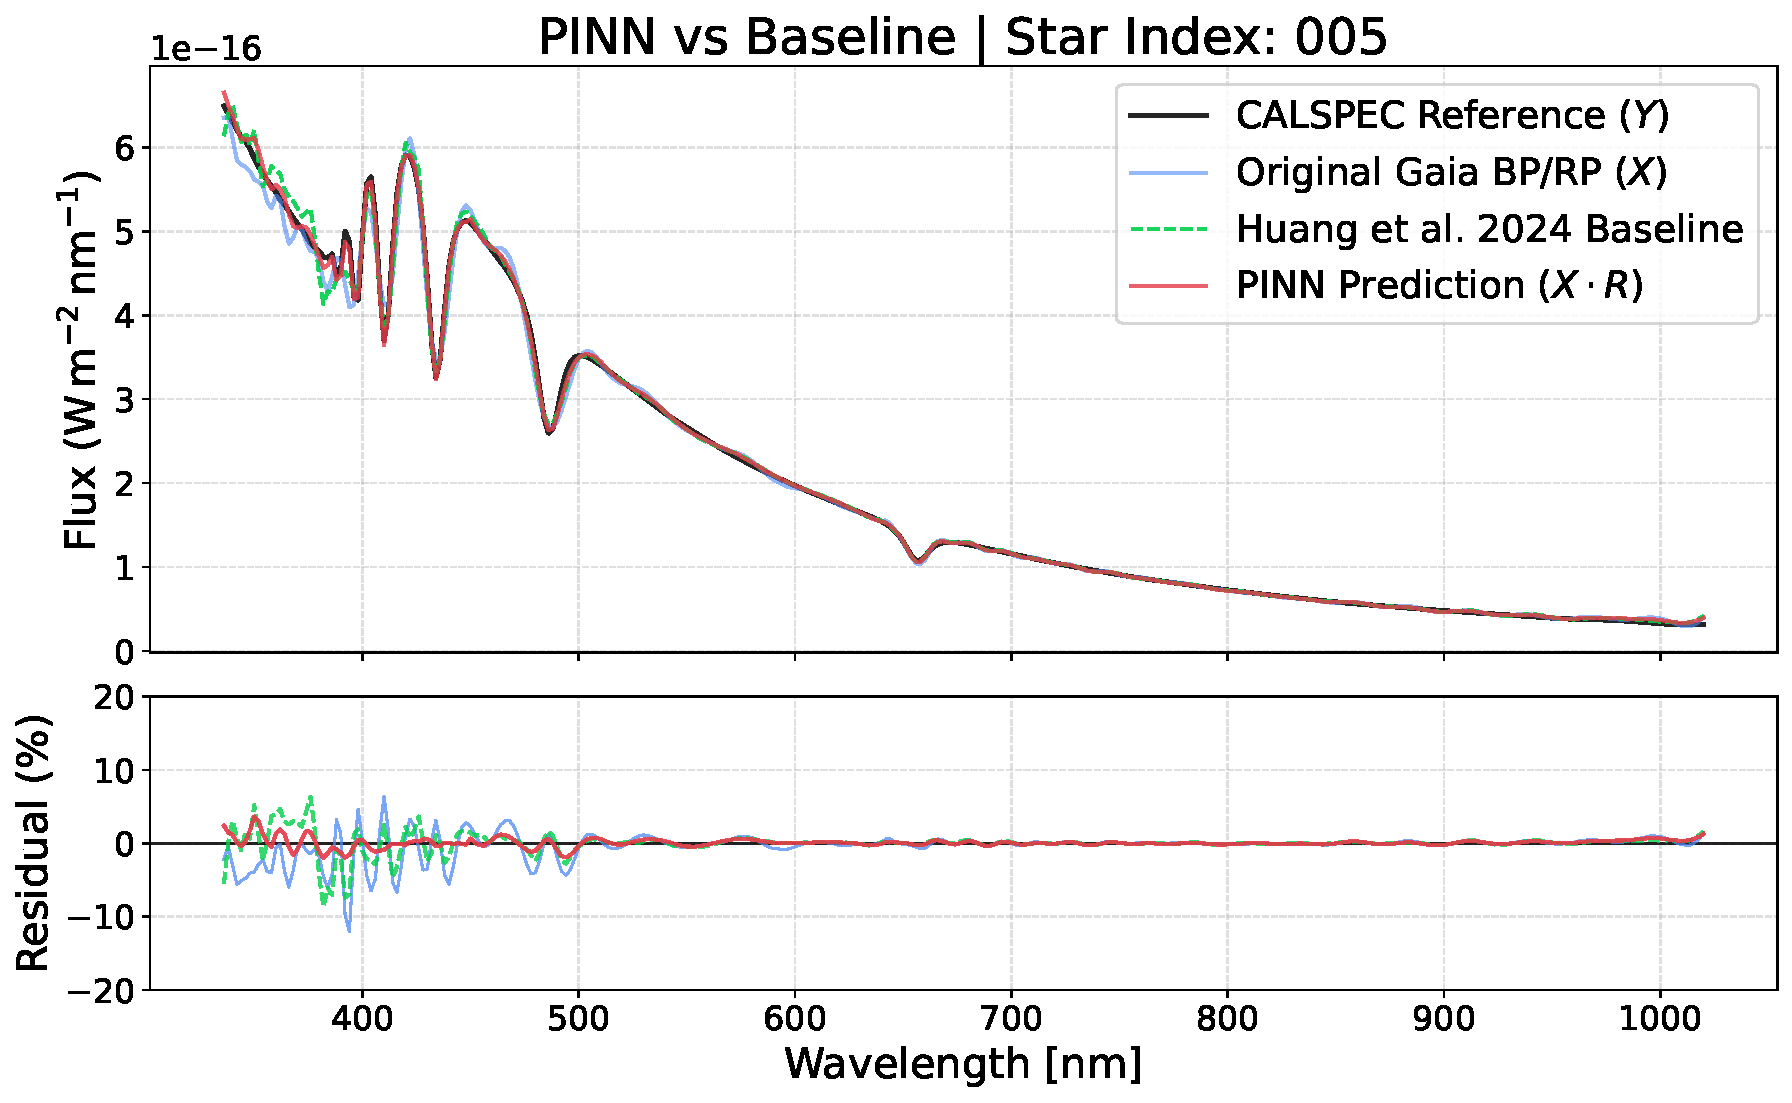
\includegraphics[width=\linewidth,height=0.69\textheight,keepaspectratio]{star_comparison_test_003.pdf}
    \column{.36\textwidth}
      \begin{itemize}
        \item Ejemplo de reconstrucción: comparación de Gaia, CALSPEC y la
              predicción de la PINN.
        \item La red especializada aborda los artefactos del borde azul
              ($<450$ nm).
        \item La validación también evalúa la respuesta en función de la
              longitud de onda.
      \end{itemize}
      \vspace{0.4em}
      \begin{beamercolorbox}[wd=\linewidth,sep=0.65em,rounded=true]{block body}
        {\scriptsize Ejemplo individual; las cifras globales se resumen en
        la diapositiva anterior.}
      \end{beamercolorbox}
  \end{columns}
\end{frame}

\begin{frame}{Comprobación independiente y límites del modelo}
  \begin{columns}[T,onlytextwidth]
    \column{.58\textwidth}
      \centering
      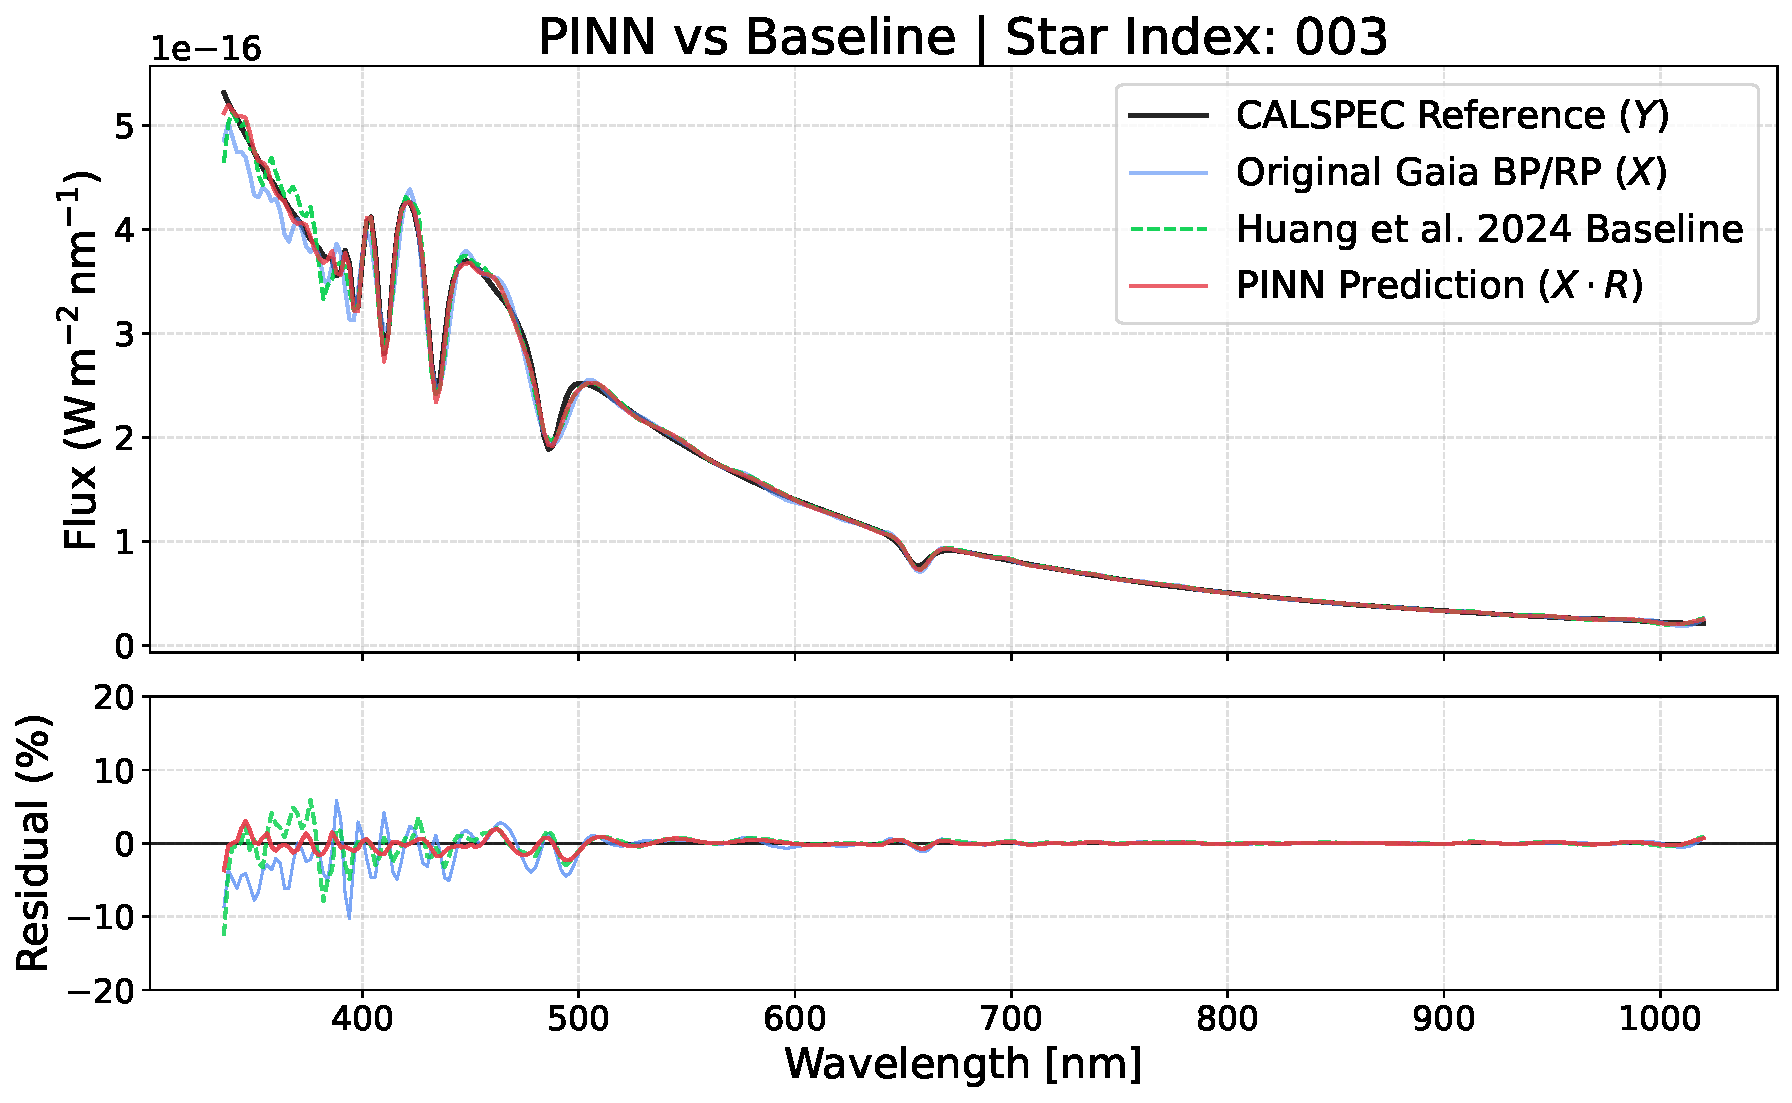
\includegraphics[width=\linewidth,height=0.42\textheight,keepaspectratio]{star_comparison_test_002.pdf}
      \par\vspace{0.1em}
      {\scriptsize\centering Prueba ciega: ejemplo representativo.\par}
    \column{.38\textwidth}
      \metric{10 estrellas}{prueba independiente retenida}
      \vspace{0.05em}
      \metric{0,495\,\%}{PN-MAE en prueba ciega}
      \vspace{0.05em}
      \metric{0,99968}{similitud espectral}
      \vspace{0.08em}
      \begin{beamercolorbox}[wd=\linewidth,sep=0.35em,rounded=true]{block body}
        {\scriptsize\color{Alert}\bfseries Límite}\par
        {\scriptsize CALSPEC cubre pocas estrellas frías: no extrapolar fuera
        del dominio de color calibrado. Ampliar las referencias.}
      \end{beamercolorbox}
  \end{columns}
\end{frame}

\begin{frame}{Aportaciones, aprendizaje y siguientes pasos}
  \begin{columns}[T,onlytextwidth]
    \column{.53\textwidth}
      \begin{block}{Aportación técnica}
        Pipeline reproducible desde los catálogos hasta la evaluación;
        arquitectura híbrida PINN--BlueWiggleNet y validación frente a
        datos no vistos.
      \end{block}
      \begin{itemize}
        \item Matemáticas aplicadas a un problema real de astrofísica.
        \item Tratamiento crítico de observaciones ruidosas e incompletas.
        \item Diseño experimental, validación y comunicación de resultados.
      \end{itemize}
    \column{.42\textwidth}
      \begin{beamercolorbox}[wd=\linewidth,sep=0.85em,rounded=true]{block body}
        {\color{ULLNavy}\bfseries Próximos pasos}\par\vspace{0.35em}
        Ampliar la muestra, especialmente con estrellas frías; contrastar
        referencias complementarias como LOWLIB y adaptar el entrenamiento
        a futuras observaciones de Gaia.
      \end{beamercolorbox}
      \vspace{0.65em}
      {\small\color{Muted}La mejora observada depende de la calidad y cobertura
      de los estándares disponibles.}
  \end{columns}
\end{frame}

\begin{frame}[plain]
  \begin{tikzpicture}[remember picture,overlay]
    \fill[ULLNavy] (current page.south west) rectangle (current page.north east);
    \fill[ULLGold] (current page.north west) rectangle ([yshift=-0.12cm]current page.north east);
  \end{tikzpicture}
  \vfill
  \centering
  {\color{ULLGold}\Large PRÁCTICAS EXTERNAS \textbar\ IAC -- ULL\par}
  \vspace{0.9cm}
  {\color{white}\Huge Gracias\par}
  \vspace{0.35cm}
  {\color{white!82}\Large ¿Preguntas?\par}
  \vfill
  {\color{white!70}\small Yaiza María Martín Mesones \hfill Curso 2026/2027\par}
  \vspace{0.5cm}
\end{frame}

\end{document}
